\section{Method}
\subsection{Problem Formulation}
At iteration $t$, the scene is a set $\mathcal{G}_t=\{G_i\}_{i=1}^{N_t}$ of anisotropic Gaussians with position, scale, rotation, opacity, and spherical-harmonic appearance. Standard alpha compositing renders a pixel by depth-ordering contributing Gaussians and computing
\begin{equation}
  C(\mathbf{p})=\sum_{i} T_i\alpha_i c_i,\qquad
  T_i=\prod_{j<i}(1-\alpha_j).
\end{equation}
Training minimizes the implementation's photometric objective, $\mathcal{L}=0.8\mathcal{L}_1+0.2(1-\mathrm{SSIM})$, while density control proposes clone and split operations. Let $A_t$ and $R_t$ be PyTorch allocated and reserved memory, $B_{\rm hard}$ the controller limit, $B_{\rm safe}$ the safety margin, and $B_{\rm np}$ a non-PyTorch allowance. The controller's available headroom is
\begin{equation}
H_t=\max\!\left(0,B_{\rm hard}-B_{\rm safe}-[\max(A_t,R_t)+B_{\rm np}]\right).
\label{eq:headroom}
\end{equation}
This is a process-level control quantity; it is not equal to whole-device VRAM.

For SH degree three, each Gaussian has 59 FP32 values (236 B). The training model counts parameters, gradients, and two Adam moments, giving $c_p=944$ B/Gaussian. Profiling fits affine transient costs
\begin{align}
M_{\rm clone}(n)&=o_c+n\mu_c c_p, & \mu_c&=1.204584,\\
M_{\rm split}(n)&=o_s+n\mu_s c_p, & \mu_s&=2.573835,
\end{align}
where $o_c=60{,}231{,}489$ B and $o_s=124{,}401{,}559$ B. The held-out largest-batch combined MAPE is 3.57\%; consequently, the model is an empirical predictor rather than a proof of physical boundedness.

\subsection{Headroom-Constrained Inflow and Allocation}
Density control forms clone and split candidate sets from accumulated view-space gradients and scale. With $C_{\min}=5{,}000$, $C_{\max}=15{,}000$, and target headroom $H^*=1{,}024$ MiB, the dynamic item cap is
\begin{equation}
C_t=\min\!\left(C_{\rm mem},
C_{\min}+\left\lfloor\alpha_t(C_{\max}-C_{\min})\right\rfloor\right),
\end{equation}
where $\alpha_t=0$ when $H_t\le H^*$ and otherwise $\min(1,(H_t-H^*)/H^*)$. $C_{\rm mem}$ is the number of worst-case-cost items that fit after fixed overhead and padding. The static ablation instead uses $\min(C_{\min},C_{\rm mem})$.

Each candidate $i$ has compensated spatial demand $d_i$ and operation cost $c_i$. After reserving a feasible split share up to $\kappa=0.40$ when the byte budget permits, the allocator sorts remaining candidates by
\begin{equation}
\lambda_i=d_i/c_i
\end{equation}
and greedily admits operations until either the transient-byte or item cap is reached. If the requested batch does not fit, the controller first prunes lowest-demand candidates; if this cannot create enough headroom, it shrinks the batch by binary search.

\subsection{Pressure-Triggered Preservation}
The evaluated lifecycle factor compares two operational policies. \emph{Eager hygiene} applies opacity and size eviction at every 100-step density-control cycle independently of admission. The implementation includes age and post-reset exceptions in this path. \emph{Pressure-triggered preservation}, used by the best configuration, instead places low-opacity and bottom-utility Gaussians in the removable pool but executes removal only for \texttt{PRUNE-FIRST} or \texttt{SHRINK-AND-PRUNE-FIRST}. Thus an under-optimized Gaussian survives while headroom suffices and can continue receiving gradient updates (Fig.~\ref{fig:lifecycle}).

Crucially, the winning preservation configuration does \emph{not} test an explicit maturity threshold: although the codebase stores a birth iteration and exposes $\tau_{\rm age}=500$, that test belongs to the eager-hygiene branch and is not consulted by the preservation cells. We therefore treat preservation as admission-coupled deferred eviction, not as a proven developmental-age model.

\begin{figure}[t]
  \centering
  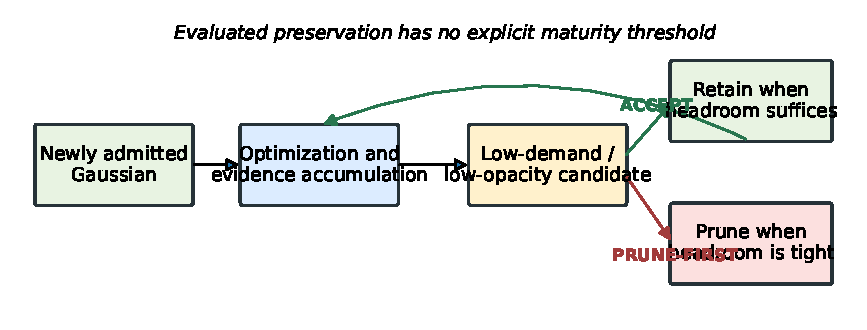
\includegraphics[width=\columnwidth]{figures/fig2_lifecycle.pdf}
  \caption{Operational lifecycle in the evaluated preservation configuration. Retention is conditional on headroom, with no explicit age threshold.}
  \label{fig:lifecycle}
\end{figure}

\begin{algorithm}[t]
\caption{Peak-VRAM-constrained mutation cycle}
\label{alg:method}
\small
\begin{algorithmic}[1]
\Require $\mathcal{G}_t$, clone/split masks, demand $d$, memory state
\State compute $H_t$ by Eq.~\eqref{eq:headroom} and affine costs
\State compute static or dynamic inflow cap $C_t$
\If{requested transient cost exceeds $H_t$}
  \State prune lowest-demand removable Gaussians
  \State recompute headroom and shrink batch if required
\EndIf
\State rank feasible candidates by $d_i/c_i$
\State enforce population cap and feasible split share $\kappa$
\State execute selected clones, then selected splits
\State log internal memory, admissions, rejections, and population
\end{algorithmic}
\end{algorithm}

\subsection{Complexity and Memory}
With $N$ active Gaussians and $K$ mutation candidates, demand and masks require $O(N)$ work and storage; sorting costs $O(K\log K)$ time and $O(K)$ temporary storage. Admission arithmetic and the 32-step shrink search are $O(1)$ in $N$. The base model stores an 8-B birth-iteration integer per Gaussian for the alternate eager-hygiene path, but pressure-triggered preservation itself adds no maturity metadata. These bounds exclude rasterization, whose tile lists depend on image content and view geometry.

\begin{table}[t]
\centering\scriptsize
\caption{Controller complexity beyond differentiable rendering.}
\label{tab:complexity}
\begin{tabular}{lcc}
\toprule
Component & Time & Auxiliary space\\
\midrule
Demand/masks & $O(N)$ & $O(N)$\\
Candidate sorting & $O(K\log K)$ & $O(K)$\\
Admission/shrink & $O(1)$ & $O(1)$\\
Birth index (optional path) & -- & 8 B/Gaussian\\
\bottomrule
\end{tabular}
\end{table}
